\documentclass[11pt,a4paper]{article}
\usepackage[T1]{fontenc}
\usepackage[margin=2.3cm]{geometry}
\usepackage{amsmath,amssymb}
\usepackage{graphicx}
\usepackage[dvipsnames]{xcolor}
\usepackage{enumitem}
\usepackage[colorlinks=true,linkcolor=blue,urlcolor=blue]{hyperref}
\setlength{\parskip}{0.6em}
\setlength{\parindent}{0pt}
\begin{document}

\begin{center}{\LARGE\bfseries openneuralnet}\\[0.4em]{\large Train a neural network from scratch and watch backpropagation, in three sessions.}\\[0.2em]\small PAN IIT OSS explainer \textbullet{} higher secondary to advanced undergraduate (levels 4-6)\end{center}

\section*{Why this exists}
A neural network is a stack of simple neurons whose settings are found, not typed. This explainer shows the mathematics behind that, a weighted sum, a bend, the chain rule and gradient descent, so you can build it yourself.

\section*{The end goal}
Train a neural network from scratch and watch backpropagation. The end goal is to train a neural network from scratch and watch backpropagation: the gradient of every weight computed by the chain rule, checked against finite differences, and a decision boundary that bends as the loss falls. The same idea sits inside large networks for images and language.

\section*{How the three sessions build up}
\begin{enumerate}[nosep]
\item \textbf{Session 1: A neuron, a line and a nudge} (Level 1, conceptual interactive model, 60 min).
\item \textbf{Session 2: Gradient descent, the sigmoid and the XOR wall} (Level 2, mathematical engineering model, 75 min).
\item \textbf{Session 3: Backpropagation: train a two-layer network} (Level 3, simulation and validation, 90 min).
\end{enumerate}

\section{Session 1: A neuron, a line and a nudge}

\subsection*{A. Real-world problem}
A traditional program is a list of rules a person wrote: if the email contains this word, mark it as spam. Machine learning turns this around: you show the computer many examples with the right answers and it finds the rules itself. The smallest learning machine is a single artificial neuron. Given two numbers about a point (say two measurements of a flower), it must say group A or group B. Can it find, from examples alone, a rule that gets all ten examples right?

\subsection*{B. Concept and theory}
A neuron has inputs x1 and x2, weights w1 and w2 and a bias b. It first computes the weighted sum z = w1 x1 + w2 x2 + b, then fires (output 1) if z \textgreater{} 0 and stays silent (output 0) otherwise. The place where it changes its mind is z = 0, which is a straight line in the (x1, x2) plane; points on one side fire, points on the other side do not. Learning by the perceptron rule: look at one example at a time. If the neuron is right, change nothing. If it is wrong, nudge: add (label - output) times the point to the weights and (label - output) to the bias. A missed group A point (label 1, output 0) adds the point, pulling the line towards it. A wrongly fired group B point (label 0, output 1) subtracts the point, pushing the line away. This is general education about how learning machines work.

\begin{itemize}[nosep]
\item x1, x2: the two inputs (measurements) of a point (no unit (any consistent unit))
\item w1, w2: weights: how much each input counts (no unit)
\item b: bias: a head start or handicap (no unit)
\item z: weighted sum w1 x1 + w2 x2 + b (no unit)
\item t: label: the right answer, 1 (group A) or 0 (group B) (no unit)
\end{itemize}

\begin{equation*}
z = w_1 x_1 + w_2 x_2 + b,\qquad \text{output} = \begin{cases}1 & z > 0\\ 0 & z \le 0\end{cases}
\end{equation*}

\begin{equation*}
\text{decision line: } w_1 x_1 + w_2 x_2 + b = 0 \;\Rightarrow\; x_2 = -\frac{w_1 x_1 + b}{w_2}
\end{equation*}

\begin{equation*}
\mathbf w \leftarrow \mathbf w + (t - \text{output})\,\mathbf x,\qquad b \leftarrow b + (t - \text{output})
\end{equation*}

\begin{center}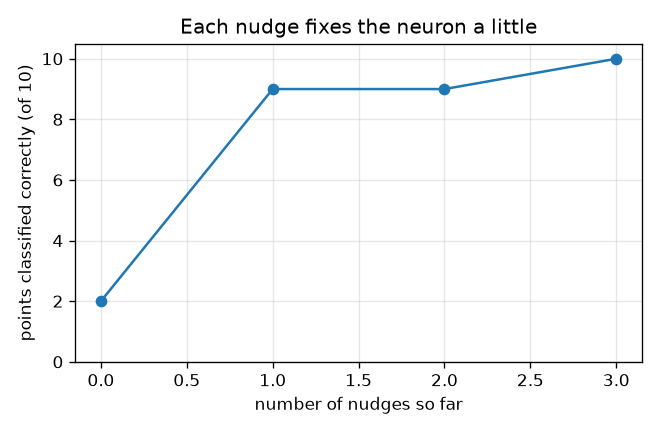
\includegraphics[width=0.85\linewidth]{figures/s01_correct_vs_nudges.png}\\\small Points classified correctly after each nudge: 2, 9, 9, 10.\end{center}

\subsection*{E. Worked example}
Start with w = (1, -2), b = 0 and apply the perceptron rule, visiting the points in the order of the table, until every point is right.
\begin{enumerate}[nosep]
\item Point 1 is (2, 2.5) with label 1. Its sum is z = 1*2 + (-2)*2.5 + 0 = -3, so the neuron is silent: wrong. At the start 2 of the 10 points are right.
\item Nudge 1: output 0, label 1, so w = (1, -2) + (1 - 0)*(2, 2.5) = (3, 0.5) and b = 0 + 1 = 1. Now 9 of 10 are right.
\item Points 2 to 7 are right. Point 8 is (0.5, -0.5) with label 0 but z = 3*0.5 + 0.5*(-0.5) + 1 = 2.25 \textgreater{} 0, so it fires wrongly.
\item Nudge 2: output 1, label 0, so w = (3, 0.5) - (0.5, -0.5) = (2.5, 1) and b = 1 - 1 = 0. Point 8 now has z = 0.75, still wrong; the count stays at 9.
\item In the next pass point 8 gives nudge 3: w = (2.5, 1) - (0.5, -0.5) = (2, 1.5) and b = -1. Now all 10 points are right and nothing more changes.
\end{enumerate}
\textbf{Answer.} After 3 nudges the neuron has w = (2, 1.5), b = -1 and classifies 10 of 10 points correctly (2, 9, 9, 10 points right after nudges 0, 1, 2, 3). The dividing line is 2 x1 + 1.5 x2 = 1.

\subsection*{F. Questions}
\begin{enumerate}[nosep]
\item \textbf{Conceptual.} What is the difference between a traditional program and a machine learning model, and why does the neuron need a bias b in addition to the weights?
\item \textbf{Numerical.} The learned neuron has w = (2, 1.5) and b = -1. What are z and the output for the new point (-0.5, -1.5)? Is that correct if this point is from group B?
\item \textbf{Graph and simulation interpretation.} In the 'points right versus bias' graph with w = (1, 1), over which range of b are all 10 points right, and why does the curve have flat steps?
\item \textbf{Design and optimisation challenge.} Design: keep w = (1, 1) and pick a bias that classifies all ten points correctly while staying as far as possible from both groups. Which b, and why?
\end{enumerate}

\section{Session 2: Gradient descent, the sigmoid and the XOR wall}

\subsection*{A. Real-world problem}
A spam filter should not only say yes or no; it should say how sure it is, for example 'this message is 90 percent likely to be spam', and it should learn its settings by a rule we can check. How do we turn a score into a probability, how do we measure how wrong the probabilities are, and how do we change the weights to be less wrong? And is there a pattern, as simple as 'exactly one of two switches is on', that a single neuron can never learn? This is general education about learning algorithms, not a tool for real decisions.

\subsection*{B. Concept and theory}
Part 1: the perceptron convergence theorem. Add a constant 1 to every input and put the bias into the weights. If some line separates the data with margin gamma (smallest distance of any point to it, for unit-length weights) and all inputs have length at most R, the perceptron rule started from zero makes at most (R / gamma)\textasciicircum{}2 updates and then stops. Part 2: the sigmoid s(z) = 1 / (1 + e\textasciicircum{}(-z)) squeezes a score into (0, 1); its derivative is s' = s (1 - s), at most 0.25. Part 3: logistic regression models the probability of label 1 as p = s(w.x + b) and measures the error by the cross-entropy loss L = -mean(y ln p + (1 - y) ln(1 - p)). Its gradient is wonderfully simple: dL/dw = mean((p - y) x) and dL/db = mean(p - y). Gradient descent repeats w = w - lr * dL/dw, where lr is the learning rate. Part 4: the learning rate. On the one-weight loss L = w\textasciicircum{}2, a step gives w = (1 - 2 lr) w, which shrinks only if lr \textless{} 1. Part 5: XOR. The labels are 0 for (0,0) and (1,1), and 1 for (0,1) and (1,0). For any line the sums z satisfy z(0,0) + z(1,1) = z(0,1) + z(1,0) (because the weighted sum is linear); if both label-1 points fire, the right side is above 0, so z(0,0) and z(1,1) cannot both be at most 0, and one label-0 point fires wrongly. So no line gets all four right.

\begin{itemize}[nosep]
\item t: label in the perceptron rule, +1 or -1 (no unit)
\item R, gamma: largest input length and margin of the data (same unit as the inputs)
\item z: score w.x + b (no unit)
\item s(z): sigmoid of the score, read as a probability (no unit)
\item p, y: predicted probability of label 1, and the true label (0 or 1) (no unit)
\item L: cross-entropy loss, averaged over the examples (no unit)
\item lr: learning rate (step size) (no unit)
\end{itemize}

\begin{equation*}
\text{updates} \le \left(\frac{R}{\gamma}\right)^2
\end{equation*}

\begin{equation*}
s(z)=\frac{1}{1+e^{-z}},\qquad s'(z)=s(z)\,\bigl(1-s(z)\bigr)
\end{equation*}

\begin{equation*}
L=-\frac1N\sum_i\bigl[y_i\ln p_i+(1-y_i)\ln(1-p_i)\bigr],\quad p_i=s(\mathbf w\cdot\mathbf x_i+b)
\end{equation*}

\begin{equation*}
\frac{\partial L}{\partial \mathbf w}=\frac1N\sum_i (p_i-y_i)\,\mathbf x_i,\qquad \frac{\partial L}{\partial b}=\frac1N\sum_i (p_i-y_i)
\end{equation*}

\begin{equation*}
\mathbf w \leftarrow \mathbf w-\text{lr}\,\frac{\partial L}{\partial \mathbf w},\qquad w_{k+1}=(1-2\,\text{lr})\,w_k \;\text{ for } L=w^2
\end{equation*}

\begin{center}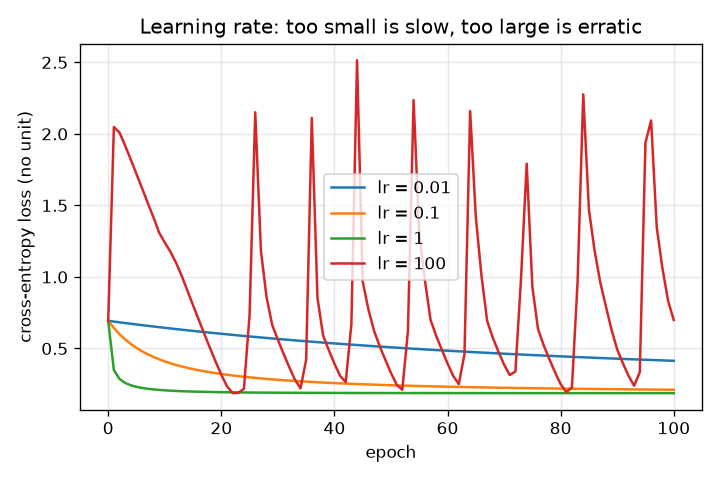
\includegraphics[width=0.85\linewidth]{figures/s02_learning_rates.png}\\\small Loss against epoch for four learning rates: too small is slow, too large is erratic.\end{center}

\subsection*{E. Worked example}
One example: input x = (2, -1) with label 0. Start with w = (0, 0), b = 0. Do one gradient descent step with learning rate 0.4 and check the loss falls.
\begin{enumerate}[nosep]
\item Score z = 0, so p = s(0) = 0.5 and the loss is -ln(1 - 0.5) = 0.6931.
\item Gradient: (p - y) x = 0.5 * (2, -1) = (1, -0.5) and (p - y) = 0.5 for the bias.
\item Step: w = (0, 0) - 0.4 * (1, -0.5) = (-0.4, 0.2) and b = 0 - 0.4 * 0.5 = -0.2.
\item New score z = (-0.4)*2 + 0.2*(-1) + (-0.2) = -1.2, so p = s(-1.2) = 0.2315.
\item New loss = -ln(1 - 0.2315) = 0.2633. The loss fell from 0.6931 to 0.2633, and the probability of label 1 fell from 0.5 to 0.23, as wanted.
\end{enumerate}
\textbf{Answer.} After one step w = (-0.4, 0.2), b = -0.2, p = 0.2315 and the loss falls from 0.6931 to 0.2633.

\subsection*{F. Questions}
\begin{enumerate}[nosep]
\item \textbf{Conceptual.} Why do we use the smooth sigmoid with cross-entropy loss for gradient descent, instead of the step 'fire if z \textgreater{} 0' of Session 1 with the count of wrong answers as the loss?
\item \textbf{Numerical.} For the single example x = (2, -1), label 0, starting from w = (0, 0), b = 0 with lr = 0.4: what are the gradient and the weights after one step? Check that the loss fell.
\item \textbf{Graph and simulation interpretation.} In the learning-rate figure, lr = 100 reaches loss 0.2 around epoch 22 and yet ends at 0.699. What does that tell you about judging a learning rate?
\item \textbf{Design and optimisation challenge.} Design: on the 100-point blob data (sep 3, seed 0) choose a learning rate and the smallest number of epochs that gets the loss to 0.2 or below and keeps it there up to epoch 100. Give a choice and a reason, and say what goes wrong with lr = 0.01 and lr = 100.
\end{enumerate}

\section{Session 3: Backpropagation: train a two-layer network}

\subsection*{A. Real-world problem}
A single neuron draws one straight line, so it cannot solve XOR or separate two interleaved spirals. Stack neurons in two layers and the decision curve can bend around the spirals. But the network has hundreds of weights: how do we get the slope of the loss for every one of them, cheaply and correctly? Backpropagation is the chain rule from calculus arranged to reuse work, and the finite-difference gradient check tells us whether we wrote it correctly. This is general education about neural networks, not a tool for real decisions.

\subsection*{B. Concept and theory}
Take N examples X (N rows, 2 columns) with labels y. Layer 1: Z1 = X W1 + b1, hidden activations H = phi(Z1) with phi = tanh (slope 1 - tanh\textasciicircum{}2). Layer 2: Z2 = H W2 + b2, output P = sigmoid(Z2). Loss L = -mean(y ln P + (1 - y) ln(1 - P)). Backpropagation applies the chain rule from the output backwards. At the output, the sigmoid and the cross-entropy combine (Session 2) into dZ2 = (P - y) / N. Then dL/dW2 = H\textasciicircum{}T dZ2 and dL/db2 = the column sum of dZ2. Pass the error back: dH = dZ2 W2\textasciicircum{}T, and through the hidden bend dZ1 = dH * phi'(Z1) (elementwise product). Then dL/dW1 = X\textasciicircum{}T dZ1 and dL/db1 = the column sum of dZ1. Gradient check: for each weight w, (L(w + h) - L(w - h)) / (2h) must match the backprop value; we report the largest relative error \textbar{}a - n\textbar{} / max(\textbar{}a\textbar{} + \textbar{}n\textbar{}, 1e-12). Optimisers: SGD w = w - lr g; momentum v = beta v + g, w = w - lr v; Adam keeps running averages m and v of g and g\textasciicircum{}2, with bias correction, and steps lr * m\_hat / (sqrt(v\_hat) + eps). Failure modes: all-zero weights keep every hidden neuron identical (no symmetry breaking); a learning rate that is too high makes the loss explode; a deep sigmoid network multiplies slopes of at most 0.25 layer after layer, so the gradient at the first layers vanishes; with many hidden neurons and few noisy points the network memorises (training accuracy 1.00, test accuracy much lower).

\begin{itemize}[nosep]
\item X, y: inputs (N rows, 2 columns) and labels (0 or 1) (no unit)
\item W1, b1, W2, b2: weights and biases of layer 1 (2 by h, h) and layer 2 (h by 1, 1) (no unit)
\item H: hidden activations phi(X W1 + b1) (no unit)
\item P: output probability sigmoid(H W2 + b2) (no unit)
\item dZ2, dZ1: gradient of the loss with respect to the pre-activations of layer 2 and 1 (no unit)
\item lr, beta, b1, b2: learning rate, momentum factor (0.9), Adam averaging factors (0.9 and 0.999) (no unit)
\item h: number of hidden neurons (count)
\end{itemize}

\begin{equation*}
Z_1 = XW_1 + b_1,\quad H = \tanh Z_1,\quad Z_2 = HW_2 + b_2,\quad P = \sigma(Z_2)
\end{equation*}

\begin{equation*}
L = -\frac1N\sum_i\bigl[y_i\ln P_i + (1-y_i)\ln(1-P_i)\bigr]
\end{equation*}

\begin{equation*}
dZ_2 = \frac{P - y}{N},\qquad \frac{\partial L}{\partial W_2} = H^{\mathsf T} dZ_2,\qquad \frac{\partial L}{\partial b_2} = \sum_i (dZ_2)_i
\end{equation*}

\begin{equation*}
dZ_1 = \bigl(dZ_2\,W_2^{\mathsf T}\bigr)\odot\bigl(1-H^2\bigr),\qquad \frac{\partial L}{\partial W_1} = X^{\mathsf T} dZ_1,\qquad \frac{\partial L}{\partial b_1} = \sum_i (dZ_1)_i
\end{equation*}

\begin{equation*}
\text{rel. error}=\frac{|a-n|}{\max(|a|+|n|,\,10^{-12})},\qquad n=\frac{L(w+h)-L(w-h)}{2h}
\end{equation*}

\begin{equation*}
m\leftarrow \beta_1 m+(1-\beta_1)g,\;\; v\leftarrow \beta_2 v+(1-\beta_2)g^2,\;\; w\leftarrow w-\text{lr}\,\frac{m/(1-\beta_1^t)}{\sqrt{v/(1-\beta_2^t)}+\epsilon}
\end{equation*}

\begin{center}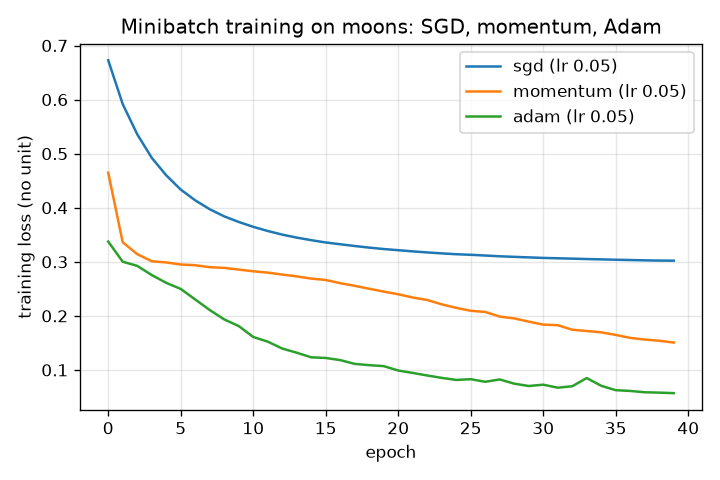
\includegraphics[width=0.85\linewidth]{figures/s03_optimisers.png}\\\small Minibatch training on moons: SGD, momentum and Adam, loss against epoch.\end{center}

\subsection*{E. Worked example}
A 2-2-1 tanh network has W1 = [[0.5, -0.3], [0.2, 0.4]], b1 = (0, 0), W2 = (0.6, -0.4)\textasciicircum{}T, b2 = 0. For the one example x = (1, 0) with label y = 1 compute the forward pass, the loss and the gradients dL/dW2 and dL/dW1 by hand.
\begin{enumerate}[nosep]
\item Layer 1: Z1 = x W1 = (0.5, -0.3). H = tanh Z1 = (0.4621, -0.2913).
\item Layer 2: Z2 = 0.6*0.4621 + (-0.4)*(-0.2913) = 0.3938, P = sigmoid(0.3938) = 0.5972, loss = -ln 0.5972 = 0.5155.
\item Output error (N = 1): dZ2 = P - y = -0.4028. So dL/dW2 = H\textasciicircum{}T dZ2 = (-0.1861, 0.1173).
\item Pass back: dH = dZ2 W2\textasciicircum{}T = (-0.2417, 0.1611). The tanh slopes are 1 - H\textasciicircum{}2 = (0.7865, 0.9151), so dZ1 = (-0.1901, 0.1474).
\item dL/dW1 = x\textasciicircum{}T dZ1: the first row is (-0.1901, 0.1474) and the second row is 0 because x2 = 0. The gradient check on this network gives a relative error of about 1e-11, well below 1e-6.
\end{enumerate}
\textbf{Answer.} P = 0.5972, loss 0.5155, dL/dW2 = (-0.1861, 0.1173), dL/dW1 = [[-0.1901, 0.1474], [0, 0]]; the numbers match the code and a finite-difference check.

\subsection*{F. Questions}
\begin{enumerate}[nosep]
\item \textbf{Conceptual.} Why does the gradient check use two-sided differences and a relative error, and what does it tell you if the error is 1e-2 instead of 1e-9?
\item \textbf{Numerical.} An output neuron gives P = 0.8 for a point with label 1 and the hidden activations are H = (0.5, -0.5), with N = 1. Find dZ2, dL/dW2 and the loss.
\item \textbf{Graph and simulation interpretation.} In the gradient-norm figure, what is the ratio of the first-layer to the last-layer gradient norm for a 10-layer sigmoid network, and for tanh and ReLU? What does it say about training the first layers?
\item \textbf{Design and optimisation challenge.} Design (mini-project): on the two-moons data (400 points, noise 0.25, seed 11, 25 percent test) choose the smallest number of hidden neurons among 2, 4, 16 that reaches 0.92 test accuracy, and say what is lost by making the network larger than needed.
\end{enumerate}

\section{Real-world mini-project}
\textbf{Classify a synthetic two-class data set and report the confusion matrix.} A lab gives you 400 points of the two-moons data set with noise 0.25 (\texttt{make\_moons(400, 0.25, 11)}). Split it 75 percent training and 25 percent test with \texttt{split(X, y, 0.25, 0)}. Train a network with \texttt{init\_params([2, h, 1], 0)}, Adam, learning rate 0.02, batch size 32 and 300 epochs for h = 2, 4 and 16 hidden neurons. The test accuracy must reach at least 0.92. This is general education about classification, not a decision tool.

\section{The path ahead}
\begin{enumerate}[nosep]
\item \textbf{Session 4: Softmax and three classes.} A network with a softmax output trained on a three-arm spiral data set.
\item \textbf{Session 5: Fight overfitting.} The same 100-hidden-neuron network on the 40 noisy points, with a regulariser.
\item \textbf{Session 6: Learn faster.} A training loop with a decaying learning rate on the spiral data.
\item \textbf{Session 7: Deep and stable.} A 20-hidden-layer sigmoid network with batch normalisation.
\item \textbf{Session 8: Build the Target animation.} A GIF with the decision boundary, the loss and accuracy curves and the hidden-layer view side by side.
\end{enumerate}

\section{Answers and hints}

\subsection*{Session 1}
\begin{enumerate}[nosep]
\item \textbf{Conceptual.} Hint: Who writes the numbers? And what happens to the line when b = 0? Solution: In a traditional program a person writes the rules. In machine learning a person writes only the form of the rule (here: weighted sum and threshold) and the numbers in it (weights, bias) are found from labelled examples. Without a bias the line w1 x1 + w2 x2 = 0 always passes through the origin, so it cannot separate two groups that are both on the same side of the origin. The bias slides the line without turning it.
\item \textbf{Numerical.} Hint: Compute z = w1 x1 + w2 x2 + b and fire only if z \textgreater{} 0. Solution: z = 2*(-0.5) + 1.5*(-1.5) + (-1) = -1 - 2.25 - 1 = -4.25, which is not above 0, so the neuron is silent (output 0): correct for group B. The number has no unit because the inputs are just numbers.
\item \textbf{Graph and simulation interpretation.} Hint: For w = (1, 1) the sum z is x1 + x2 + b. Group A sums are at least 4.5 and group B sums are at most 0. Solution: Group A needs x1 + x2 + b \textgreater{} 0 for the smallest group A sum (4.5), so b \textgreater{} -4.5. Group B needs x1 + x2 + b \textless{}= 0 for the largest group B sum (0), so b \textless{}= 0. All ten are right for -4.5 \textless{} b \textless{}= 0 (for example b = -2). The curve is a staircase because the count is a whole number that changes only when the line passes over a point.
\item \textbf{Design and optimisation challenge.} Hint: The allowed range from question C is -4.5 \textless{} b \textless{}= 0; the groups are closest to the line at its two ends. Solution: The allowed range is -4.5 \textless{} b \textless{}= 0, so the middle value b = -2.25 leaves the same room (2.25) on both sides. A line far from both groups is safer when new points arrive with a little noise. Trade-off: with a margin this wide the rule is more robust, but nothing in this data tells us where the true boundary is; any b in the range fits the ten examples equally well. I took b = -2, which also works (checked in the checkpoint).
\end{enumerate}

\subsection*{Session 2}
\begin{enumerate}[nosep]
\item \textbf{Conceptual.} Hint: What is the slope of a step function away from the jump? What would gradient descent do with a slope of 0? Solution: The step function and the count of wrong answers are flat almost everywhere: their slope is 0, so the gradient says nothing about which way to move the weights. The sigmoid is smooth and its slope s(1 - s) is positive everywhere, so a small change of a weight changes the loss by a small, measurable amount, and the gradient points downhill.
\item \textbf{Numerical.} Hint: Use (p - y) x with p = 0.5. The loss is -ln(1 - p) for label 0. Solution: p = 0.5, gradient (1, -0.5), bias gradient 0.5. New weights w = (-0.4, 0.2), b = -0.2, new score -1.2, p = 0.2315, loss 0.2633 \textless{} 0.6931. All numbers are dimensionless. Sanity check: the new p moved towards the label 0.
\item \textbf{Graph and simulation interpretation.} Hint: Compare the end of the curve with its start (ln 2 = 0.693). Solution: A step that is too long overshoots the valley: the loss can dip below a target by luck and then jump out again. After 100 epochs the loss of 0.699 is no better than the starting 0.693, so lr = 100 has not learned anything. Always look at the whole curve and the final value, not at the first time it dips below a target.
\item \textbf{Design and optimisation challenge.} Hint: Use epochs\_to\_reach(X, y, lr, 0.2) for several learning rates and look at the end of each curve. Solution: With lr = 1 the loss first reaches 0.2 after 15 epochs and settles at 0.188 after 100 epochs, so choose lr = 1 and about 15 to 20 epochs. lr = 0.1 also works but needs 156 epochs (10 times the cost). lr = 0.01 never reaches 0.2 within 500 epochs: too slow. lr = 100 touches 0.2 at epoch 22 but ends at 0.699: unstable. Trade-off: a larger rate is faster but closer to the unstable region; take a rate comfortably inside the stable range.
\end{enumerate}

\subsection*{Session 3}
\begin{enumerate}[nosep]
\item \textbf{Conceptual.} Hint: Think about the size of the error of (L(w + h) - L(w)) / h versus the two-sided version, and about gradients of very different sizes. Solution: The two-sided difference (L(w + h) - L(w - h)) / (2h) has error of order h\textasciicircum{}2, the one-sided has error of order h, so it is far more accurate. A relative error compares the size of the mismatch with the size of the gradient, so tiny gradients and big gradients are judged fairly. A relative error near 1e-9 means backprop and the numbers agree; 1e-2 means a real bug (the checkpoint shows that forgetting the tanh slope gives about 0.5).
\item \textbf{Numerical.} Hint: dZ2 = P - y, dL/dW2 = H times dZ2, loss = -ln P for label 1. Solution: dZ2 = 0.8 - 1 = -0.2. dL/dW2 = -0.2 * (0.5, -0.5) = (-0.1, 0.1). Loss = -ln 0.8 = 0.2231. Gradient descent adds to W2 a step against the gradient: W2[0] grows and W2[1] falls, which makes the output larger for this point. All values are dimensionless.
\item \textbf{Graph and simulation interpretation.} Hint: Read the two ends of each curve; the vertical axis is logarithmic. Solution: For sigmoid the first layer has a gradient about 1.3e-6 times that of the last layer (7e-8 versus 6e-2): the early layers barely learn, the vanishing gradient. For tanh the ratio is about 0.36 and for ReLU about 0.35: the early layers still receive a usable gradient (with these initialisations: scale sqrt(1 / fan\_in) for tanh, sqrt(2 / fan\_in) for ReLU). At 20 sigmoid layers the ratio is about 2e-13.
\item \textbf{Design and optimisation challenge.} Hint: Train h = 2, 4 and 16 with Adam, lr 0.02, batch 32, 300 epochs and compare the test accuracy and the train-test gap. Solution: h = 2 reaches only 0.83 (too little capacity: two hidden neurons cannot bend the boundary enough), h = 4 reaches 0.96 and h = 16 reaches 0.97. The smallest h that passes is 4. A bigger network costs more computation and, on few noisy points, more risk of memorising (Session 3 overfitting experiment: 100 hidden neurons give training accuracy 1.00 and test accuracy 0.80 on 40 points). Assumption: one fixed seed, so a different split could change the third digit.
\end{enumerate}

\section{How to join}
Read \texttt{CONTRIBUTING.md} in the repository, then pick an issue labelled \texttt{good first issue}. Repository: \url{https://github.com/KrunalPanchal1995/openneuralnet}

\end{document}
